\section {Architecture}

The system comprises three types of roles, which may be physically distributed on different machines.

\begin{figure}[h!]
  \centering
    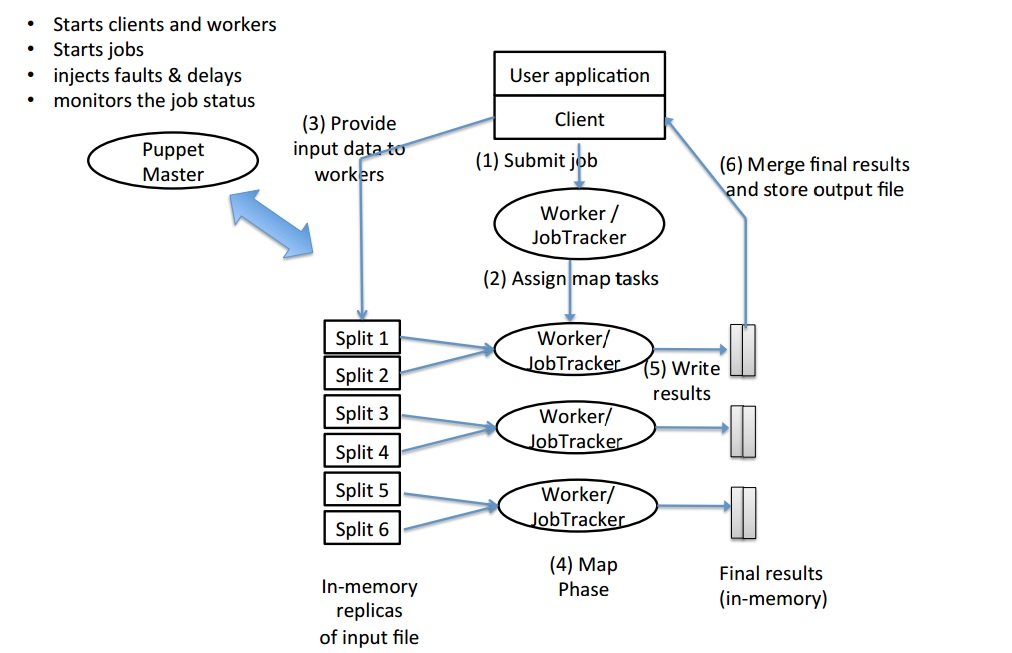
\includegraphics[width=0.5\textwidth]{pictures/PADIMapNoReduceArchitecture.jpg}
    \caption{}
\end{figure}


%%%%%%%%%%%%%%%%%%%%%%%%%%%%%%%%%%%%%%%%%%%%%%%%%%%
\subsection {Application API and Clients }

\textbf{Application API} - submits map jobs to the system

\textbf{Client} - is physically co-located with the user-level application and exposes to user-level applications a method to submit jobs in the system. Also exports two services, which are used by the other nodes in PADIMapNoReduce platform to communicate with the client:

\vspace*{8pt}%
- Provide splits to the workers

- Receive the output data when processing is finished
\vspace*{8pt}%


%%%%%%%%%%%%%%%%%%%%%%%%%%%%%%%%%%%%%%%%%%%%%%%%%%%%
\subsection {Worker/Job Tracker}




%%%%%%%%%%%%%%%%%%%%%%%%%%%%%%%%%%%%%%%%%%%%%%%%%%%%
\subsection {Puppet Master}
This component of the system serves only for testing purposes, allowing not only to inject failures/delays in the system, but also create instances of the worker processes and submit jobs. Each machine used by PADIMapNoReduce must have its own puppet master associated.
